% Drawing 85/03-2 -- folder 85, batch 03, archive page 55 (PDF page 56).
% Transcription: dans la marge gauche, un petit triangle : « $s$ » au sommet du haut, « $a$ » le long du côté gauche, « $f'$ » à l'intérieur
% Kind: triangle with labels s, a, f'. Method 2 (schematic redraw from the facsimile). Status: ok.
% Notes: Ink, two faint pencil strokes inside. Triangle with s at the top vertex, a beside the left side and f' inside. Redrawn 2026-11-12 (issue 128): to check again.
% Coordinates: 1 unit = 1 mm = 1/100 of the crop width (bbox in page fractions: [0.1, 0.18, 0.28, 0.28]).
% Redrawn by Claude (claude-fable-5-2), issue #128, 2026-11-12; not checked by a human; not compiled (no TeX in the session).
% Rights: reproduces part of the work -- behind RENDER_TRANSCRIPTS, never published by itself.
\documentclass[tikz,border=3pt]{standalone}
\usepackage{amsmath,amssymb}
\usetikzlibrary{patterns,arrows.meta}
\tikzset{pencil/.style={black!45}, struck/.style={black!35}, mpt/.style={circle,draw,inner sep=1.3pt}, pt/.style={circle,fill,inner sep=0.9pt}, opt/.style={circle,draw,fill=white,inner sep=1.1pt}}
\begin{document}
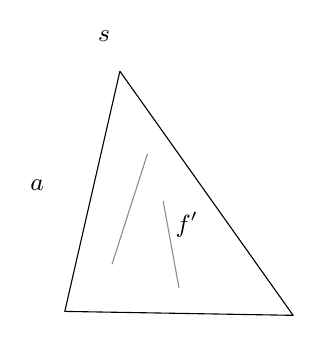
\begin{tikzpicture}[x=1mm,y=1mm,line cap=round,line join=round,font=\scriptsize]
\draw (43.5,-30.5) -- (36.5,-61) -- (65.5,-61.5) -- (43.5,-30.5);
\draw[pencil] (42.5,-55) -- (47,-41);
\draw[pencil] (51,-58) -- (49,-47);
\node[inner sep=1pt] at (41.5,-26) {\small $s$};
\node[inner sep=1pt] at (33,-45) {\small $a$};
\node[inner sep=1pt] at (52,-50) {\small $f'$};
\end{tikzpicture}
\end{document}
